\documentclass[12pt]{article}

\usepackage[utf8]{inputenc}
\usepackage[T1]{fontenc}
\usepackage{sbc-template}
\usepackage{graphicx,url}
\usepackage[brazil]{babel}
\usepackage{booktabs}
\usepackage{amsmath,amssymb}
\usepackage{multirow}

\sloppy

\title{Modelagem em Grafos de Coocorrência e Detecção de Comunidades na Base Histórica da Assembleia Nacional Constituinte de 1988: Da Curadoria dos Dados à Descoberta de Eixos Temáticos}

% --- MODO DOUBLE-BLIND (SUBMISSÃO BRASNAM) ---
\author{Autores omitidos para revisão duplamente cega}
\address{Afiliação e endereços eletrônicos omitidos para revisão duplamente cega}

% --- DESCOMENTAR NA VERSÃO FINAL (CAMERA-READY) ---
% \author{Rafael Roseira Machado\inst{1}, André Luiz Satoshi Kawamoto\inst{1}}
% \address{Departamento Acadêmico de Computação\\
%   Universidade Tecnológica Federal do Paraná (UTFPR) -- Campo Mourão, PR -- Brasil
%   \email{rafaroseira27@outlook.com, kawamoto@utfpr.edu.br}
% }

% Macro para o link do repositório (trocar no camera-ready):
\newcommand{\repolink}{\textit{[link do repositório público omitido para revisão duplamente cega]}}
% \newcommand{\repolink}{\url{https://github.com/alkawamo/base-saic}}

\begin{document}

\maketitle

\begin{abstract}
  During the drafting of the 1988 Brazilian Constitution, the Federal Senate's Informatics Center (Prodasen) digitized 72,719 letters sent by citizens into the Constituent Information Support System (SAIC). Despite its historical value, the raw dataset suffers from severe structural anomalies, lack of sender disambiguation, and an unbalanced top-down thematic classification into 24 macro-themes. This paper presents two main contributions: (i) the complete curation, standardization, and public release of the SAIC database, including sender disambiguation into 64,869 unique citizens via Fuzzy Matching; and (ii) a bottom-up thematic reanalysis based on a word co-occurrence network weighted by Positive Pointwise Mutual Information (PPMI) and partitioned via the Louvain algorithm. Removing edges below the 95th PPMI percentile ($\text{min\_df} = 2\%$) yields a connected network of 322 terms and 1,823 edges with high modularity ($Q = 0.6363$), organized into 8 thematic communities. Quantitative cross-tabulation against the original 1986 catalog shows where the official taxonomy succeeded (e.g., Educational Policy and State Political Structure) and where it failed---most notably by omitting a dedicated macro-theme for Public Security and the Penal System, diluting massive popular demands into generic legal categories. The curated dataset and analysis scripts are publicly available at \repolink.
\end{abstract}

\begin{resumo}
  Durante a elaboração da Constituição Brasileira de 1988, o Centro de Informática e Processamento de Dados do Senado Federal (Prodasen) digitou 72.719 cartas enviadas por cidadãos no Sistema de Apoio Informático à Constituinte (SAIC). Embora de inestimável valor histórico, a base bruta apresenta graves anomalias estruturais, ausência de identificação única de remetentes e uma classificação temática top-down desequilibrada em 24 macrotemas. Este artigo apresenta duas contribuições principais: (i) a curadoria completa, padronização e disponibilização pública da base SAIC, incluindo a desambiguação de remetentes em 64.869 cidadãos únicos via Fuzzy Matching; e (ii) uma reanálise temática bottom-up baseada em redes de coocorrência de palavras ponderadas por Positive Pointwise Mutual Information (PPMI) e particionadas pelo algoritmo de Louvain. A poda de arestas no percentil 95 de PPMI ($\text{min\_df} = 2\%$) produz uma rede conexa de 322 termos e 1.823 arestas com alta modularidade ($Q = 0,6363$), estruturada em 8 comunidades temáticas. A matriz de contingência quantitativa frente ao catálogo de 1986 evidencia onde a taxonomia oficial acertou (Política Educacional e Estrutura Política do Estado) e onde falhou --- sobretudo ao omitir um macrotema para Segurança Pública e Sistema Penal, diluindo uma expressiva demanda popular em categorias jurídicas genéricas. A base de dados tratada e os scripts utilizados estão disponíveis em \repolink.
\end{resumo}

\section{Introdução}

No final da década de 1980, em meio ao processo de redemocratização após duas décadas de regime militar, a Assembleia Nacional Constituinte assumiu a incumbência de redigir a Constituição Brasileira de 1988. Além do debate parlamentar, promoveu-se uma iniciativa inédita de participação popular direta: cinco milhões de formulários impressos foram distribuídos em agências dos Correios, prefeituras e assembleias legislativas para que os cidadãos enviassem sugestões ao texto constitucional \cite{monclaire1991,agenciasenado2024}. Para processar esse acervo, o Centro de Informática e Processamento de Dados do Senado Federal (Prodasen) criou, em 1986, o Sistema de Apoio Informático à Constituinte (SAIC) \cite{senado1988}, reunindo 72.719 cartas e formulários digitados.

Apesar de constituir um patrimônio único da história política brasileira, a utilização científica da base SAIC esbarra em dois obstáculos fundamentais. O primeiro é de \textbf{qualidade e integridade de dados}: a base bruta apresenta falhas severas de codificação (\textit{encoding}), deslocamento estrutural de conteúdos entre colunas (subtemas inseridos no campo de catálogo, fragmentos de cartas no campo de indexação e temas alocados no campo de destinatário), registros corrompidos por fórmulas de planilhas eletrônicas e ausência de um identificador único para cada cidadão remetente.

O segundo obstáculo é de \textbf{natureza metodológica e taxonômica}. Na década de 1980, a equipe do Prodasen classificou manualmente as cartas seguindo uma abordagem \textit{top-down} (pré-fixada) em 24 macrotemas (\textit{Catálogo}), desdobrados em 1.308 subtemas (\textit{Indexação}). Conforme apontado já por \cite{monclaire1991}, essa categorização mistura rubricas extremamente amplas --- como \textit{Direito --- Organização do Estado} (25.243 cartas) e \textit{Organização Social} (23.555 cartas) --- com categorias hiperespecíficas de baixíssima frequência, como \textit{Política Nacional da Informática} (282 cartas) e \textit{Política Sanitária} (454 cartas). Ademais, tentativas recentes de agrupar essas cartas no nível do documento inteiro via modelos de linguagem \cite{agenciasenado2024} esbarram no fato de que os cidadãos frequentemente abordavam múltiplos assuntos em uma mesma carta, gerando um único \textit{cluster} massivo e indiferenciado de ``cartas multitemáticas''.

Para superar essas limitações, este artigo altera a unidade de análise do documento para a \textbf{rede de coocorrência de termos}, na qual uma carta multitemática contribui com arestas ponderadas conectando conceitos específicos no grafo. As principais contribuições deste trabalho são:
\begin{enumerate}
    \item \textbf{Curadoria, restauração e publicação aberta da base SAIC:} Correção de anomalias estruturais entre colunas, padronização geográfica (respeitando a divisão territorial de 1986--1987), desambiguação de remetentes via \textit{Fuzzy Matching} (identificando 64.869 cidadãos únicos) e disponibilização pública do \textit{dataset} higienizado e dos scripts de processamento em repositório aberto (\repolink);
    \item \textbf{Modelagem em grafos de coocorrência ponderados por PPMI:} Construção de uma rede semântica livre de saturação por termos frequentes, demonstrando que o corte no percentil 95 de PPMI ($\text{min\_df} = 2\%$) maximiza a modularidade ($Q = 0,6363$) mantendo a conectividade global da rede;
    \item \textbf{Contraste quantitativo e qualitativo (\textit{top-down} vs.\ \textit{bottom-up}):} Cruzamento das 8 comunidades emergentes com os 24 macrotemas do Prodasen, comprovando que a classificação oficial de 1986 omitiu um eixo dedicado a \textbf{Sistema Penal e Segurança Pública} e subestimou mobilizações corporativas organizadas (como as 2.060 cartas de detetives particulares).
\end{enumerate}

\section{Trabalhos Relacionados}

O estudo pioneiro sobre a base SAIC foi conduzido por \cite{monclaire1991}, que investigaram a composição sociológica dos remetentes, mas mantiveram sua análise temática restrita aos 24 macrotemas do Prodasen, cujas assimetrias de granularidade foram reconhecidas pelos próprios autores. Recentemente, a \cite{agenciasenado2024} aplicou técnicas de processamento de linguagem natural para projetar as cartas em mapa semântico bidimensional; contudo, ao tratar a carta inteira como unidade indivisível, a maioria dos registros concentrou-se em um bloco indiferenciado de ``cartas multitemáticas'', impedindo a extração de métricas de rede e a mensuração de conexões entre temas distintos.

Na análise computacional do discurso político, \cite{rule2015} modelaram discursos presidenciais norte-americanos (1790--2014) como redes semânticas de coocorrência de termos, aplicando o algoritmo de Louvain \cite{blondel2008} para identificar categorias discursivas emergentes. De forma complementar, \cite{erz2026} analisou a polarização no Congresso dos EUA (1873--2025) combinando modelagem de tópicos via LDA e detecção de comunidades em redes de similaridade. Diferentemente do LDA --- que exige fixar \textit{a priori} o número de tópicos --- ou de projeções de documentos inteiros, a modelagem em grafos ponderados por PPMI permite decompor as cartas em relações conceituais elementares e derivar os eixos temáticos da própria topologia da rede \cite{macanovic2022,tsai2022}.

\section{Curadoria e Higienização da Base de Dados SAIC}

A base SAIC original é composta por 72.719 linhas (cartas/formulários) e 20 colunas, abrangendo dados demográficos opcionais do remetente (nome, município, UF, CEP, sexo, local de moradia, grau de instrução, estado civil, faixa etária, faixa de renda e profissão/atividade), metadados de controle, destinatário parlamentar, as duas colunas de classificação do Prodasen (\textit{Catálogo} e \textit{Indexação}) e o texto integral da sugestão (\textit{Texto Sugestão}).

O processo de engenharia e curadoria de dados envolveu cinco etapas principais: (i)~\textbf{Padronização de \textit{encoding} e artefatos de planilha:} conversão integral para UTF-8 e substituição de marcadores espúrios e 323 erros de fórmula (\texttt{\#NOME?}) pelo valor padronizado \texttt{N/A}; (ii)~\textbf{Correção de anomalias estruturais entre colunas:} realocação de macrotemas digitados no campo \textit{Destinatário} e fragmentos de cartas inseridos em \textit{Indexação}, delimitando \textit{Catálogo} estritamente às combinações dos 24 macrotemas oficiais e consolidando \textit{Indexação} em 1.308 subtemas únicos; (iii)~\textbf{Padronização geográfica com fidelidade histórica:} harmonização de municípios (de 3.913 para 3.542 variantes) e correção de UFs para as 26 existentes em 1986--1987, preservando o território do futuro estado do Tocantins vinculado a Goiás; (iv)~\textbf{Desambiguação de nomes via \textit{Fuzzy Matching}:} agrupamento aproximado por distância de Levenshtein \cite{levenshtein1966,navarro2001} (limiar de similaridade de 90\%), reduzindo remetentes de 61.315 para 57.268 e destinatários de 2.836 para 2.193; e (v)~\textbf{Identificador único de remetente (\textit{ID Pessoa}):} chave composta \textit{(Nome, Município, UF)} \cite{monclaire1991}, atribuindo identificadores exclusivos a registros com campos nulos para evitar falsas fusões, consolidando as 72.719 cartas em \textbf{64.869 cidadãos distintos}.

A Tabela~\ref{tab:limpeza} sintetiza o impacto do tratamento nas colunas que sofreram intervenções estruturais (as demais 14 colunas demográficas e de controle mantiveram suas contagens originais de nulos e valores únicos). A base de dados tratada (\texttt{SAIC.csv}) e os scripts de limpeza e análise encontram-se publicamente disponíveis no repositório \repolink.

\begin{table}[htb]
\centering
\caption{Comparação de valores ausentes (N/A) e valores únicos antes e depois da curadoria nas principais colunas afetadas da base SAIC.}
\label{tab:limpeza}
\footnotesize
\begin{tabular}{lcccc}
\toprule
\textbf{Coluna} & \textbf{N/A (Antes)} & \textbf{N/A (Depois)} & \textbf{Únicos (Antes)} & \textbf{Únicos (Depois)} \\
\midrule
\textbf{ID Pessoa} \textit{(nova)} & --- & 0 & --- & 64.869 \\
\textbf{Nome} & 6.453 & 6.459 & 61.315 & 57.268 \\
\textbf{Destinatário} & 43.317 & 43.325 & 2.836 & 2.193 \\
\textbf{Catálogo} & 180 & 150 & 21.749 & 14.532 \\
\textbf{Indexação} & 14.253 & 1.152 & 39.482 & 42.941 \\
\textbf{Texto Sugestão} & 835 & 835$^*$ & 70.096 & 70.150 \\
\textbf{Município} & 21 & 97 & 3.913 & 3.542 \\
\textbf{UF} & 0 & 122 & 27 & 26 \\
\textbf{CEP} & 0 & 119 & 5.921 & 5.919 \\
\bottomrule
\multicolumn{5}{l}{\scriptsize $^*$Cartas com texto ausente mantidas para integridade dos metadados demográficos.}
\end{tabular}
\end{table}

\section{Metodologia de Construção e Análise da Rede de Coocorrência}

\subsection{Pré-processamento Textual e Matriz Documento-Termo Binária}

Para evitar que cartas idênticas enviadas em campanhas organizadas inflassem artificialmente as contagens de coocorrência, removeram-se inicialmente as duplicatas exatas da coluna \textit{Texto Sugestão}. Das 71.884 cartas preenchidas, 395 textos distintos repetiam-se (somando 2.129 linhas, ou 1.734 cópias excedentes, com destaque para formulários padronizados sobre ensino religioso e regulamentação profissional), resultando em $N = 70.150$ textos únicos válidos.

Cada texto foi submetido às etapas de tokenização, remoção de \textit{stopwords} e caracteres não alfabéticos, e lematização \cite{hotho2005,tan1999} utilizando o modelo pré-treinado \texttt{pt\_core\_news\_md} da biblioteca \texttt{spaCy}. Para salvaguardar a privacidade dos cidadãos (evitando a disponibilização direta de termos e assinaturas individuais presentes nas cartas em repositório aberto) e manter o repositório leve e ágil ($< 10$~MB), o cache binário de lematização não é versionado no Git. Em vez disso, disponibiliza-se o script de curadoria (\texttt{src/curate.py}) que processa os 70.150 textos e reconstrói o corpus localmente \textit{on-the-fly} em cerca de 10 a 12 minutos em CPU convencional, com persistência automática em disco para todas as análises subsequentes. Para reduzir a dimensionalidade e eliminar ruídos lexicais raros, aplicou-se um filtro de frequência documental mínima ($\text{min\_df}$), retendo apenas os $M$ termos presentes em pelo menos uma fração pré-determinada das cartas.

Em vez de utilizar a contagem bruta de frequência de palavras intra-documento, definiu-se a Matriz Documento-Termo $A$ de dimensão $N \times M$ de forma \textbf{estritamente binária}, onde $A_{k,i} \in \{0, 1\}$ registra apenas a presença ($1$) ou ausência ($0$) do termo $i$ na carta $k$. Essa escolha impede que a repetição retórica de uma mesma palavra ao longo de uma única carta distorça a estimativa de coocorrência no corpus.

A matriz simétrica de coocorrência de termos $C$ de dimensão $M \times M$ é obtida pelo produto matricial $C = A^T \cdot A$, cujo elemento $C_{i,j} = \sum_{k=1}^{N} A_{k,i} A_{k,j}$ contabiliza exatamente o número de cartas distintas nas quais os termos $i$ e $j$ coocorrem. Os elementos da diagonal principal $C_{i,i} = \text{df}(i)$ correspondem à frequência documental marginal de cada termo $i$.

\subsection{Ponderação por PPMI e Poda Topológica}

O uso direto de contagens brutas $C_{i,j}$ como peso das arestas favorece conexões espúrias entre palavras de alta frequência geral que coocorrem por mero acaso estatístico, gerando grafos excessivamente densos. Para mensurar a afinidade semântica genuína entre dois termos $i$ e $j$ ($i \neq j$), emprega-se o \textit{Positive Pointwise Mutual Information} (PPMI) \cite{church1990}:
\begin{equation}
\text{PMI}(i, j) = \log_2 \left( \frac{P(i, j)}{P(i) \cdot P(j)} \right), \quad \text{PPMI}(i, j) = \max\big(0, \text{PMI}(i, j)\big)
\end{equation}
em que a probabilidade conjunta empírica e as probabilidades marginais são estimadas sobre o total de documentos analisados ($N$):
\begin{equation}
P(i, j) = \frac{C_{i, j}}{N}, \quad P(i) = \frac{\text{df}(i)}{N} = \frac{C_{i, i}}{N}
\end{equation}

Após o cálculo do PPMI, a diagonal principal é zerada ($\text{PPMI}(i, i) = 0$) para vedar a formação de laços. Pares de termos com independência estatística ou repulsão semântica ($\text{PMI}(i,j) \le 0$) recebem peso zero e são descartados. Como vocabulários de alta frequência ainda preservam densidades elevadas mesmo sob restrição de positividade do PMI, aplica-se uma etapa adicional de poda de arestas (\textit{pruning}) baseada em um limiar de corte $\theta_p$, correspondente ao $p$-ésimo percentil da distribuição empírica dos valores positivos de PPMI. O grafo não direcionado resultante $G = (V, E)$ contém uma aresta $e = (v_i, v_j) \in E$ com peso $w(v_i, v_j) = \text{PPMI}(i, j)$ se, e somente se, $\text{PPMI}(i, j) \ge \theta_p$, descartando-se eventuais vértices isolados (grau zero).

\subsection{Detecção de Comunidades e Métricas de Centralidade}

Para identificar os eixos temáticos emergentes (\textit{bottom-up}), particiona-se o grafo ponderado $G$ por meio do algoritmo de Louvain \cite{blondel2008}, que otimiza iterativamente a \textbf{modularidade ponderada ($Q$)} da partição. Para garantir reprodutibilidade diante da natureza heurística do método, fixou-se inicialmente a semente do gerador pseudoaleatório (\texttt{seed = 42}).

Por fim, para caracterizar o papel estrutural dos termos dentro de cada eixo temático, extrai-se o subgrafo induzido $G_c = (V_c, E_c)$ de cada comunidade $c$ e calculam-se três métricas clássicas de centralidade sobre sua \textbf{topologia não ponderada} (uma vez que o filtro severo $\text{PPMI} \ge \theta_{95}$ já assegura que todas as arestas retidas em $E_c$ representam associações semânticas fortes, evitando a inversão conceitual entre peso de afinidade e custo de caminho mínimo): (i) \textbf{Centralidade de Grau}, identificando os termos mais volumosos e polissêmicos do agrupamento; (ii) \textbf{Centralidade de Intermediação (\textit{Betweenness})}, revelando os termos que atuam como pontes articuladoras entre subpautas distintas da comunidade; e (iii) \textbf{Centralidade de Proximidade (\textit{Closeness})}, apontando os conceitos com menor distância média até todos os demais termos do eixo temático \cite{kim2011,schaeffer2007,girvan2002}.

\subsection{Protocolo de Avaliação de Estabilidade Particional}

Dada a natureza heurística do algoritmo de Louvain decorrente da ordem estocástica de visitação dos vértices durante a fase de agregação local, é imperativo averiguar se a partição temática obtida decorre de propriedades intrínsecas da topologia semântica ou de mero viés de convergência local. Para tanto, executou-se um protocolo sistemático de estabilidade submetendo o grafo ótimo ($|V| = 322$, $|E| = 1.823$) a 50 execuções independentes do algoritmo com sementes pseudoaleatórias distintas ($\textit{seeds} \in [0, 49]$).

Para cada execução $s$, registraram-se a modularidade $Q_s$ e o número de comunidades $K_s$. Adicionalmente, mensurou-se a concordância composicional entre cada partição resultante e a partição canônica de referência (\textit{seed 42}) por meio de duas métricas clássicas de similaridade particional: o \textit{Normalized Mutual Information} (NMI) e o \textit{Adjusted Rand Index} (ARI), verificando se os termos permanecem consistentemente agrupados independentemente da inicialização do gerador pseudoaleatório.

\section{Experimentos, Resultados e Discussão}

\subsection{Parametrização da Rede e Maximização da Modularidade}

Avaliaram-se inicialmente cinco limiares de frequência mínima documental ($\text{min\_df} \in \{1{,}0\%;\; 1{,}5\%;\; 2{,}0\%;\; 2{,}5\%;\; 3{,}0\%\}$). Sem a poda por percentil ($\theta = 0$), embora o número de vértices caia de $709$ ($\text{min\_df} = 1{,}0\%$) para $203$ ($\text{min\_df} = 3{,}0\%$) e o de arestas de $162.432$ para $13.675$, a densidade da rede mantém-se praticamente constante entre $64{,}72\%$ e $66{,}70\%$. Esse fenômeno ocorre porque a elevação do $\text{min\_df}$ retém justamente o núcleo de palavras mais gerais e frequentes do corpus, que coocorrem intensamente entre si.

Para esparsificar a rede e revelar sua estrutura comunitária, avaliaram-se quatro percentis de corte da distribuição de PPMI ($p \in \{50, 75, 90, 95\}$) para cada $\text{min\_df}$. A Tabela~\ref{tab:poda} apresenta as dimensões topológicas, o número de componentes conexas e a modularidade $Q$ obtida pelo algoritmo de Louvain em cada cenário.

\begin{table}[htb]
\centering
\caption{Dimensões do grafo, conectividade e modularidade ($Q$) após poda de arestas por percentil de PPMI.}
\label{tab:poda}
\resizebox{\textwidth}{!}{%
\begin{tabular}{ccccccccc}
\toprule
\textbf{\texttt{min\_df}} & \textbf{Percentil} & \textbf{Corte ($\theta_p$)} & \textbf{Arestas ($|E|$)} & \textbf{Nós ($|V|$)} & \textbf{Densidade} & \textbf{Comp.\ Conexas} & \textbf{Mod.\ ($Q$)} & \textbf{Comunidades} \\
\midrule
\multirow{4}{*}{1,0\%} & 50 & 0,49 & 81.216 & 709 & 32,36\% & 1 & 0,2446 & 5 \\
 & 75 & 0,79 & 40.608 & 709 & 16,18\% & 1 & 0,3243 & 6 \\
 & 90 & 1,14 & 16.244 & 707 & 6,51\% & 1 & 0,4375 & 9 \\
 & 95 & 1,43 & 8.122 & 698 & 3,34\% & 1 & 0,5507 & 8 \\
\midrule
\multirow{4}{*}{1,5\%} & 50 & 0,46 & 39.501 & 488 & 33,24\% & 1 & 0,2591 & 5 \\
 & 75 & 0,73 & 19.751 & 488 & 16,62\% & 1 & 0,3657 & 6 \\
 & 90 & 1,04 & 7.901 & 487 & 6,68\% & 1 & 0,4853 & 7 \\
 & 95 & 1,31 & 3.951 & 477 & 3,48\% & 1 & 0,5841 & 7 \\
\midrule
\multirow{4}{*}{\textbf{2,0\%}} & 50 & 0,42 & 18.228 & 336 & 32,39\% & 1 & 0,3169 & 5 \\
 & 75 & 0,68 & 9.114 & 336 & 16,19\% & 1 & 0,4231 & 6 \\
 & 90 & 0,98 & 3.646 & 334 & 6,56\% & 1 & 0,5581 & 7 \\
 & \textbf{95} & \textbf{1,25} & \textbf{1.823} & \textbf{322} & \textbf{3,53\%} & \textbf{1} & \textbf{0,6363} & \textbf{8} \\
\midrule
\multirow{4}{*}{2,5\%} & 50 & 0,40 & 9.751 & 246 & 32,36\% & 1 & 0,3347 & 6 \\
 & 75 & 0,65 & 4.876 & 246 & 16,18\% & 1 & 0,4562 & 5 \\
 & 90 & 0,95 & 1.951 & 242 & 6,69\% & 2 & 0,5880 & 7 \\
 & 95 & 1,21 & 976 & 229 & 3,74\% & 3 & 0,6510 & 9 \\
\midrule
\multirow{4}{*}{3,0\%} & 50 & 0,39 & 6.838 & 203 & 33,35\% & 1 & 0,3113 & 5 \\
 & 75 & 0,62 & 3.419 & 203 & 16,68\% & 1 & 0,4295 & 7 \\
 & 90 & 0,91 & 1.368 & 198 & 7,01\% & 2 & 0,5838 & 7 \\
 & 95 & 1,17 & 684 & 188 & 3,89\% & 4 & 0,6707 & 9 \\
\bottomrule
\end{tabular}%
}
\end{table}

Os resultados da Tabela~\ref{tab:poda} fornecem uma justificativa objetiva para a escolha da configuração \textbf{$\text{min\_df} = 2{,}0\%$ com percentil 95 ($\theta_{95} = 1{,}25$)}: trata-se da parametrização que \textbf{maximiza a modularidade ($Q = 0,6363$) dentre todas as redes que preservam a integridade global do grafo em uma única componente conexa} (322 nós e 1.823 arestas, após o descarte de 14 vértices que ficaram com grau zero após o corte). Valores superiores de $\text{min\_df}$ ($2{,}5\%$ e $3{,}0\%$) nos percentis 90 e 95 sofrem fragmentação topológica em múltiplas componentes desconexas e perda severa de vocabulário temático. A Figura~\ref{fig:grafo} apresenta a visualização completa do grafo resultante com suas 8 comunidades e principais polos conceituais destacados.

\begin{figure}[htb]
\centering
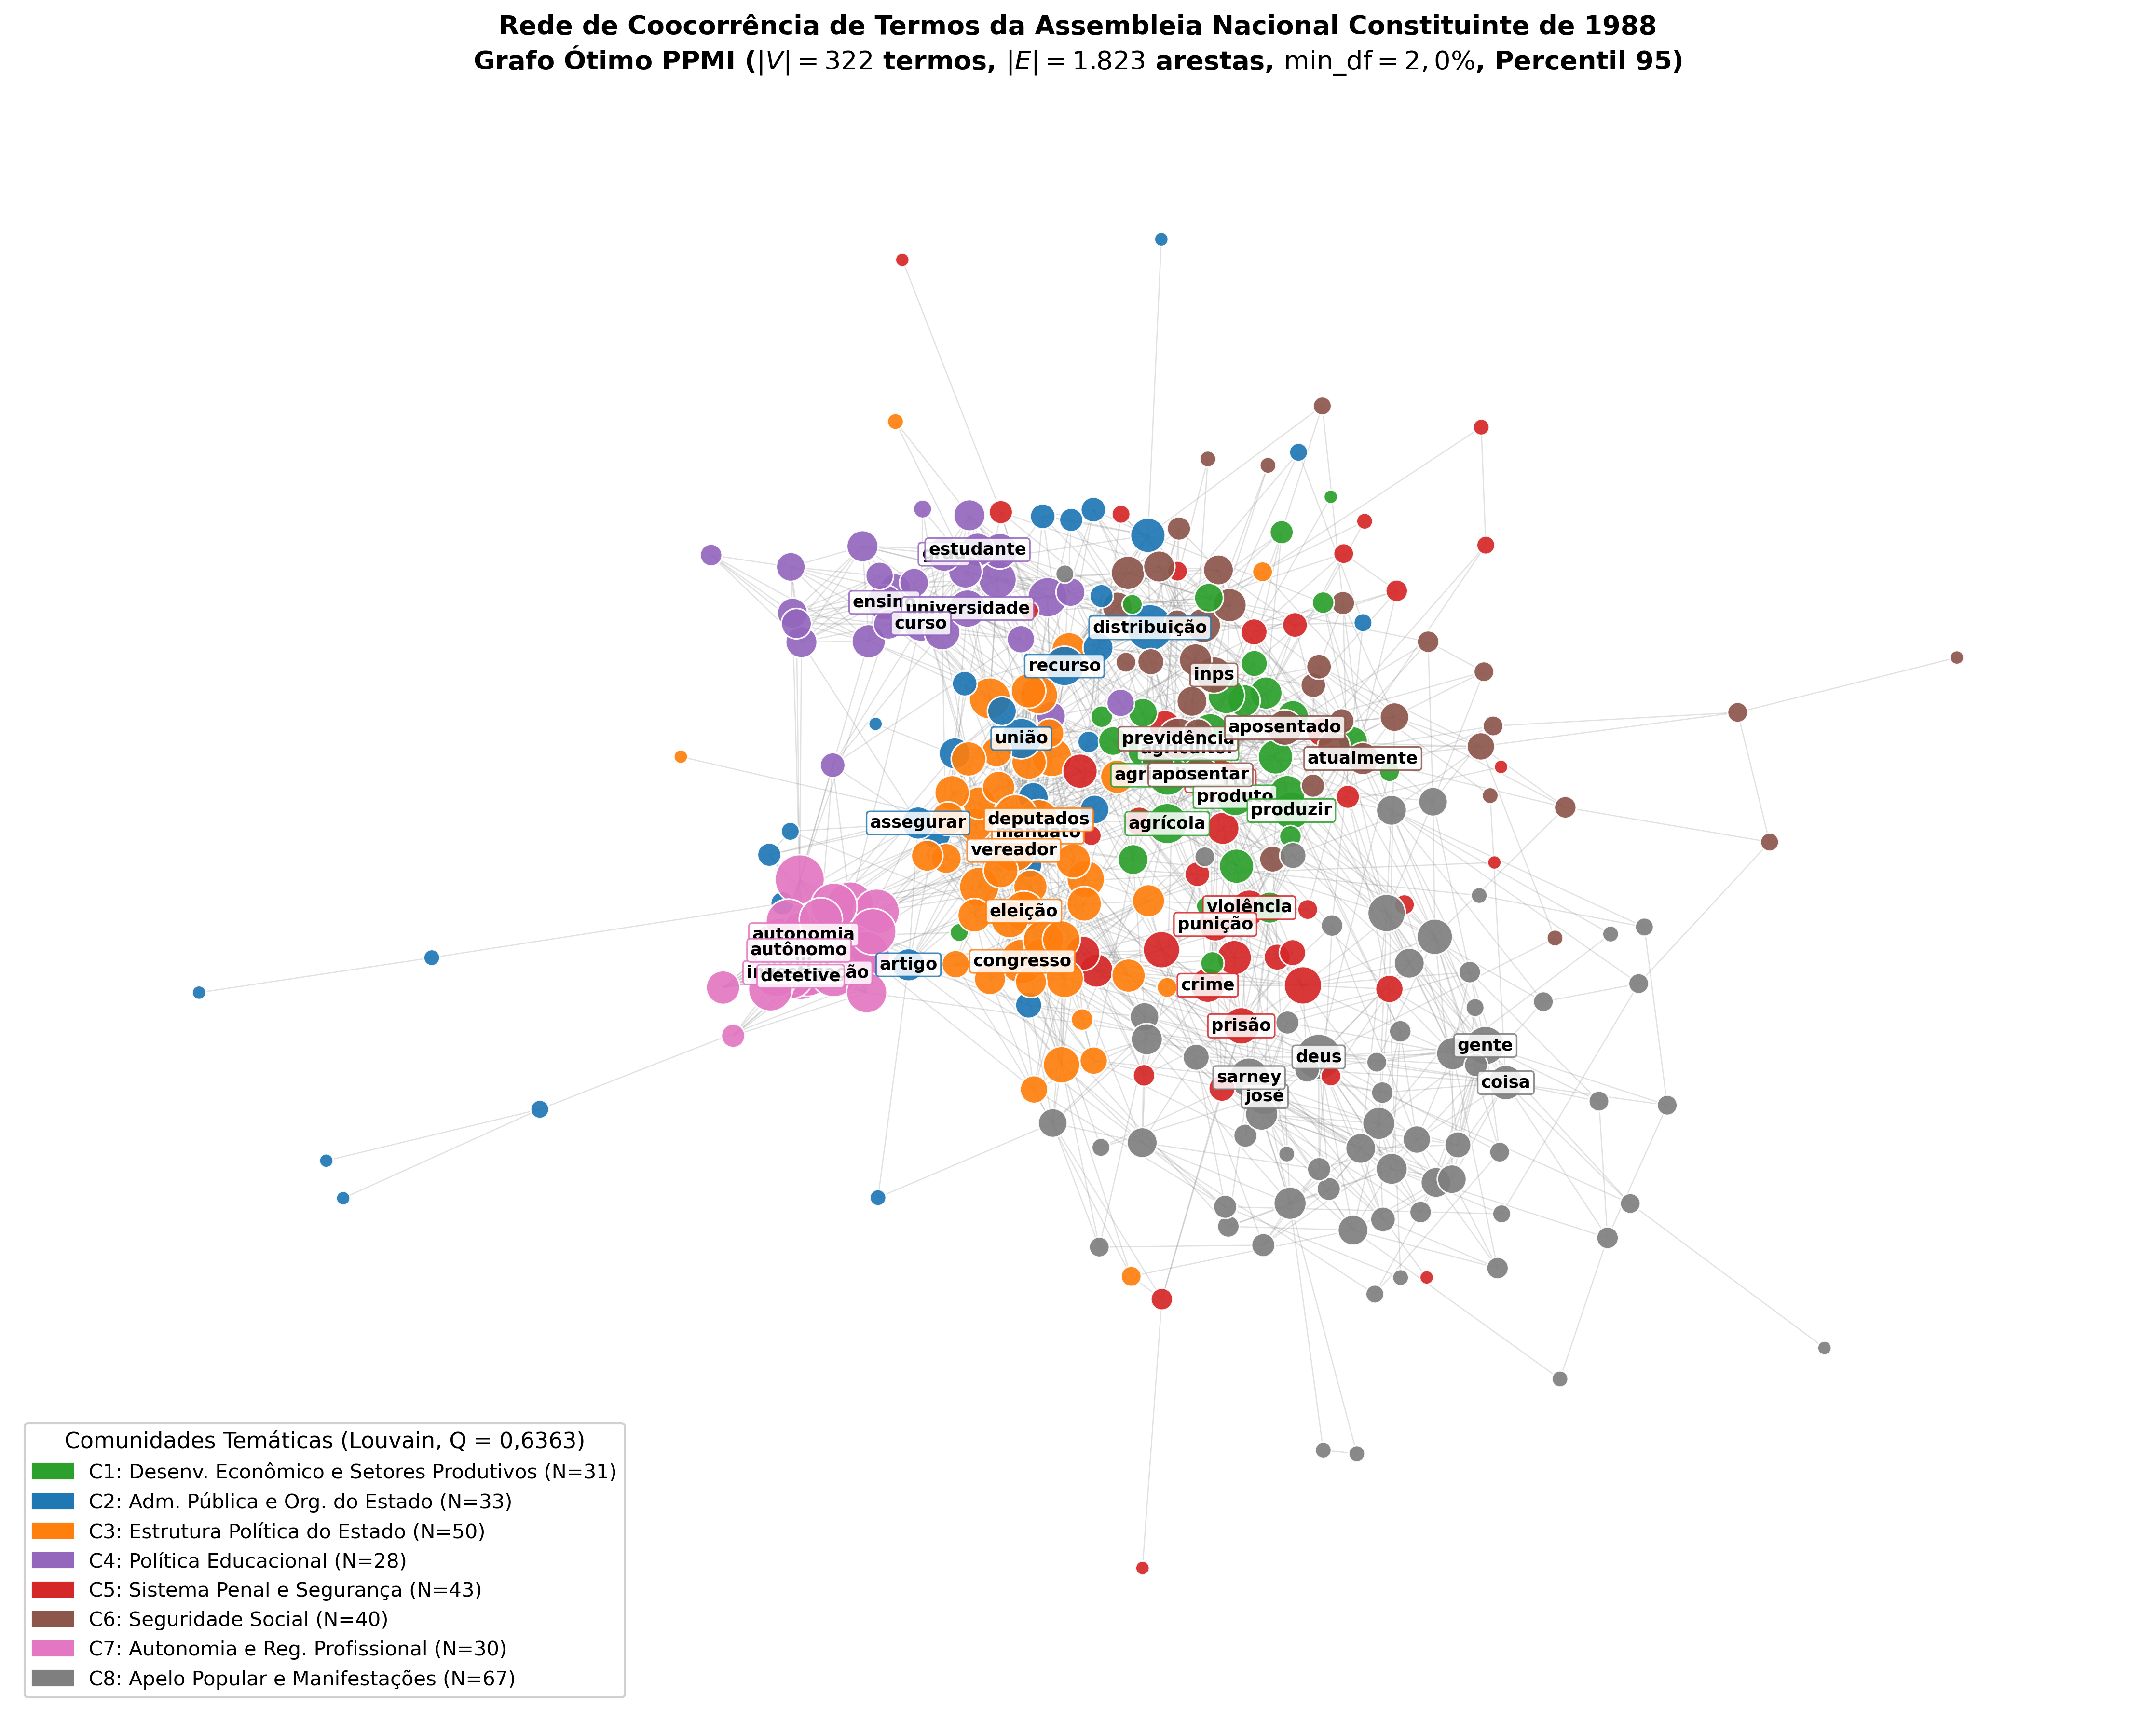
\includegraphics[width=0.85\textwidth]{grafo_comunidades_brasnam.png}
\caption{Rede de coocorrência de termos da Constituinte de 1988 ($\text{min\_df} = 2\%$, percentil 95, $Q = 0,6363$) particionada em 8 comunidades pelo algoritmo de Louvain.}
\label{fig:grafo}
\end{figure}

\subsection{Análise de Estabilidade do Algoritmo de Louvain (50 Sementes)}

Para certificar que a estrutura em 8 comunidades não decorre de viés de convergência da semente estocástica, submeteu-se o grafo ótimo a 50 execuções independentes do algoritmo de Louvain com sementes distintas ($\text{seeds} \in [0, 49]$), cujos resultados estão sintetizados na Figura~\ref{fig:estabilidade}. A partição revelou estabilidade consistente: a modularidade média atingiu $Q = 0{,}6361 \pm 0{,}0034$ (mín.\ $0{,}6215$, máx.\ $0{,}6397$, mediana $0{,}6366$), com coeficiente de variação de apenas $0{,}54\%$. A configuração modal foi $K = 8$, observada em $62\%$ das execuções (31 vezes), enquanto $K = 7$ ocorreu nas $38\%$ restantes (19 vezes), sem nenhuma ocorrência de fragmentação espúria ($K \ge 9$) ou fusão excessiva ($K \le 6$). Avaliando as 49 sementes independentes frente à partição canônica ($\text{seed } 42$), obteve-se NMI médio de $0{,}8007 \pm 0{,}0311$ (mediana $0{,}8037$) e ARI médio de $0{,}7079 \pm 0{,}0484$ (mediana $0{,}7145$), comprovando elevada concordância composicional.\footnote{Considerando todas as 50 sementes, $\text{NMI} = 0{,}8047 \pm 0{,}0415$.}

\begin{figure}[htb]
\centering
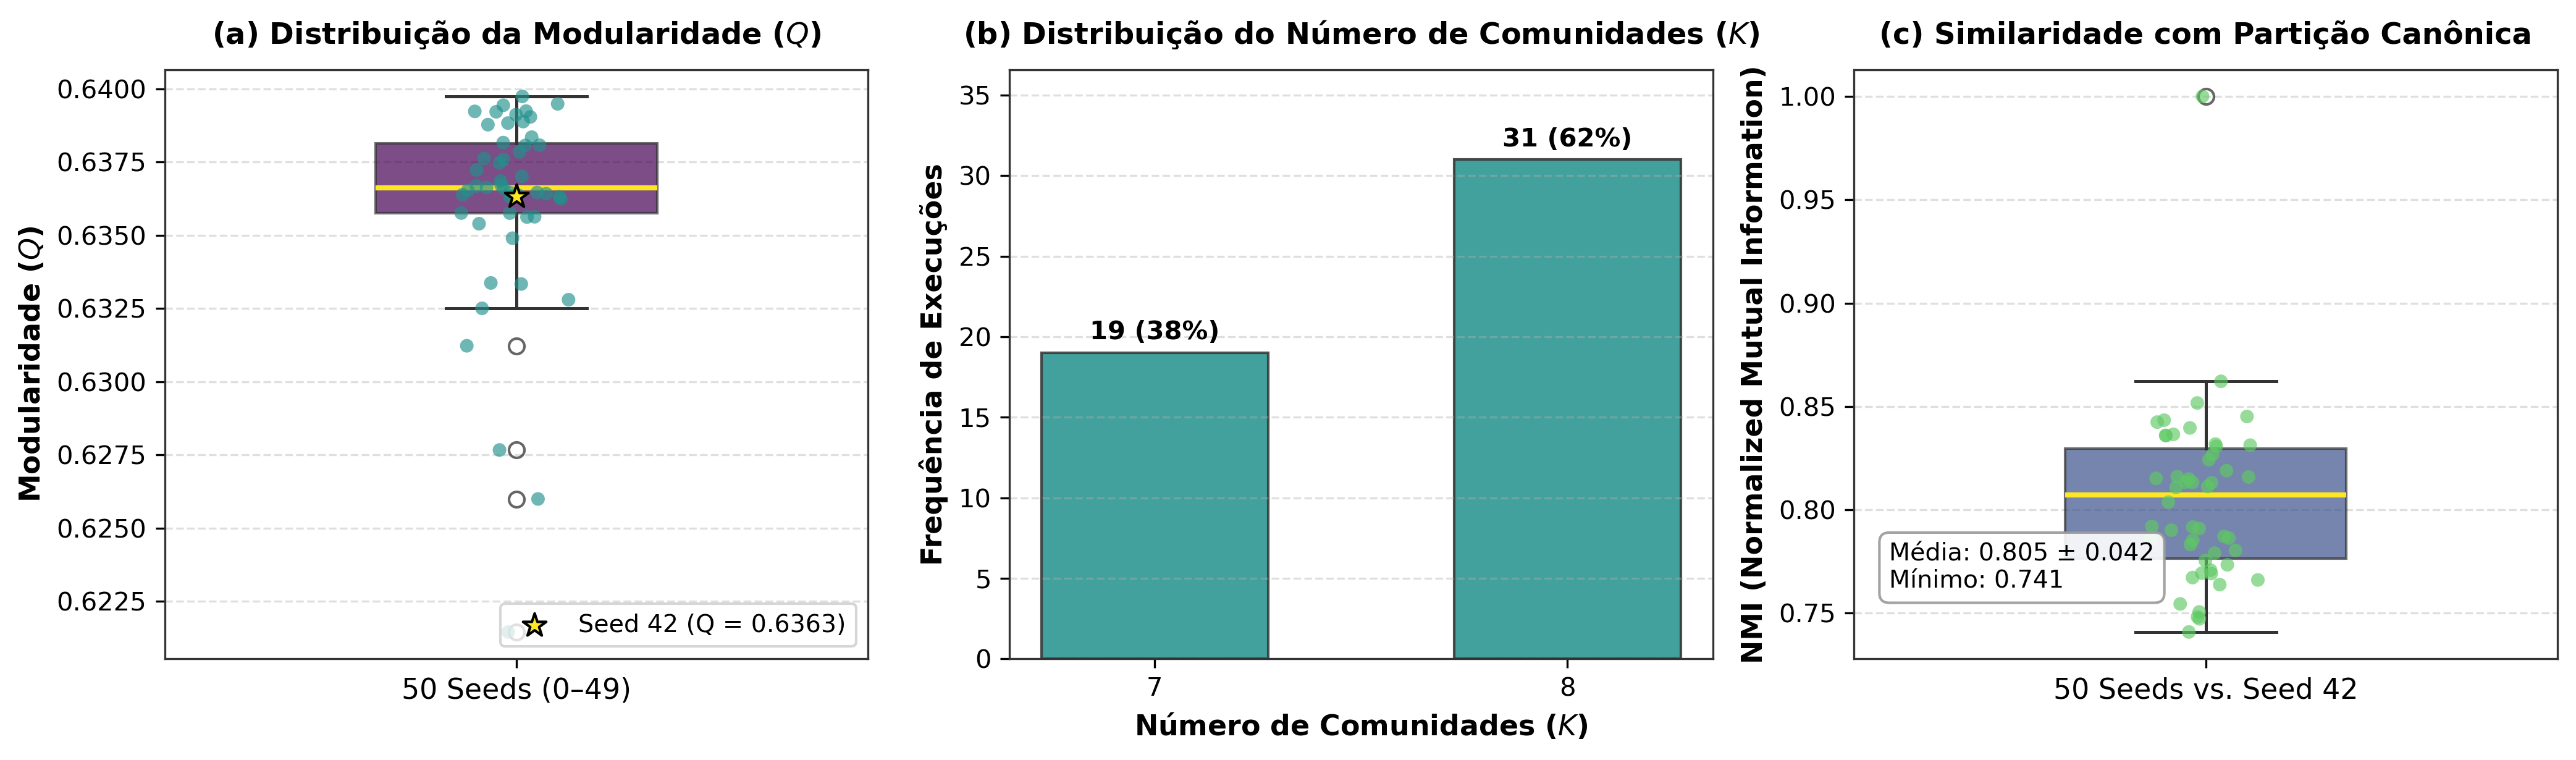
\includegraphics[width=0.85\textwidth]{fig_estabilidade_louvain.png}
\caption{Estabilidade do Louvain (50 sementes): distribuições de $Q$, $K$ e similaridade NMI frente à partição canônica.}
\label{fig:estabilidade}
\end{figure}

\paragraph{Dinâmica de Fusão $K=7$ vs.\ $K=8$ e Qualificação Estrutural.}
O rastreamento das 19 execuções com $K=7$ revelou que a contração decorre da fusão entre C1 (Desenvolvimento Econômico) e C2 (Administração Pública) em 78,9\% dos casos (15 execuções). Essa aglutinação é historicamente plausível: no contexto de 1986--1987 (Plano Cruzado e reforma agrária), regulação estatal e produção econômica operavam de forma indissociável, bifurcando-se apenas na máxima resolução de modularidade ($Q=0{,}6363$). As demais comunidades mantiveram-se invariantes, qualificando o achado como 7 macro-eixos nucleares com desdobramento setorial do bloco desenvolvimentista.

\subsection{Análise das Oito Comunidades Encontradas e Centralidades}

A partição ótima ($Q = 0,6363$) divide o vocabulário em \textbf{8 comunidades temáticas} bem delimitadas. A Tabela~\ref{tab:comunidades} sintetiza as 8 comunidades, o número de termos que compõem cada subgrafo, os vértices líderes segundo as três métricas de centralidade e a interpretação qualitativa de seu vocabulário.

\begin{table}[htb]
\centering
\caption{Síntese das 8 comunidades detectadas e líderes de centralidade em cada subgrafo.}
\label{tab:comunidades}
\footnotesize
\setlength{\tabcolsep}{4pt}
\begin{tabular}{p{3.8cm}cccp{5.8cm}}
\toprule
\textbf{Comunidade (\textit{Bottom-Up})} & \textbf{Grau} & \textbf{Interm.} & \textbf{Proxim.} & \textbf{Principais Termos e Escopo} \\
\midrule
\textbf{C1: Desenv.\ Econômico} & \textit{agricultura} & \textit{agricultura} & \textit{agricultura} & \textit{terra, reforma, preço, indústria}. Agropecuária e macroeconomia. \\
\addlinespace[2pt]
\textbf{C2: Adm.\ Pública} & \textit{união} & \textit{união} & \textit{união} & \textit{órgão, cargo, concurso, funcionário}. Burocracia estatal e funcionalismo. \\
\addlinespace[2pt]
\textbf{C3: Estrutura Política} & \textit{mandato} & \textit{congresso} & \textit{mandato} & \textit{eleição, voto, deputado, partido}. Representação parlamentar e voto. \\
\addlinespace[2pt]
\textbf{C4: Política Educacional} & \textit{ensino} & \textit{ensino} & \textit{ensino} & \textit{escola, educação, universidade, gratuito}. Ensino público e religioso. \\
\addlinespace[2pt]
\textbf{C5: Sistema Penal/Segurança} & \textit{prisão} & \textit{aborto} & \textit{violência} & \textit{crime, polícia, pena, morte}. Segurança pública e punição penal. \\
\addlinespace[2pt]
\textbf{C6: Seguridade Social} & \textit{previdência} & \textit{previdência} & \textit{previdência} & \textit{aposentadoria, hospital, assistência, salário}. Previdência, saúde e renda. \\
\addlinespace[2pt]
\textbf{C7: Regulação Profissional} & \textit{detetive} & \textit{detetive} & \textit{detetive} & \textit{profissional, liberal, detetive, particular}. Profissões e atividade autônoma. \\
\addlinespace[2pt]
\textbf{C8: Apelo Popular} & \textit{Deus} & \textit{Deus} & \textit{Deus} & \textit{fome, desemprego, pobre, Sarney}. Carestia e manifestações populares. \\
\bottomrule
\end{tabular}
\end{table}

A análise conjunta da topologia (Tabela~\ref{tab:comunidades}) revela três achados fundamentais:
\begin{enumerate}
    \item \textbf{Convergência de papéis centrais em cinco comunidades:} Em C1 (\textit{agricultura}), C2 (\textit{união}), C4 (\textit{ensino}), C6 (\textit{previdência}) e C7 (\textit{detetive}), um único vértice domina simultaneamente o grau, a intermediação e a proximidade, atuando como polo gravitacional absoluto do respectivo debate.
    \item \textbf{Diferenciação estrutural na comunidade de Sistema Penal e Segurança (C5):} C5 é a única comunidade que apresenta \textbf{três líderes distintos} para cada métrica de centralidade: \textit{prisão} detém o maior grau (conectando-se diretamente a todo o vocabulário punitivo e policial); \textit{violência} possui a maior proximidade (apresentando a menor distância média a todos os termos da comunidade, por permear tanto o debate criminal quanto o familiar); e \textit{aborto} lidera a intermediação, funcionando como nó-ponte entre o núcleo punitivo (\textit{crime, matar, pena, morte}) e o núcleo de proteção à vida e à família (\textit{criança, pai, filho, família, abandonar}).
    \item \textbf{Limitações morfológicas da lematização automática:} Observou-se nos subgrafos que o modelo \texttt{pt\_core\_news\_md} do \texttt{spaCy} manteve algumas flexões e derivações como nós distintos (ex.: \textit{deputado/deputados} em C3, \textit{querer/queremos} em C7, \textit{agrícola/agrário/agrária} em C1 e o erro de lematização \textit{peçar} para \textit{peço} em C8). Embora essa limitação morfológica infle ligeiramente a contagem de nós, o fato de todas essas variantes serem alocadas juntas em suas respectivas comunidades demonstra a robustez semântica da ponderação por PPMI.
\end{enumerate}

\subsection{Contraste Quantitativo: Catálogo \textit{Top-Down} (1986) vs.\ Comunidades \textit{Bottom-Up}}

Para validar quantitativamente a correspondência entre os 24 macrotemas do Prodasen e as 8 comunidades descobertas, construiu-se uma matriz de contingência empírica baseada na \textbf{Regra de Projeção Termo-Documento (Regra A, preferencial)}. Para cada comunidade temática $C_k$, projetam-se seus termos constitutivos sobre as cartas em que ocorrem, agregando as ocorrências segundo os macrotemas oficiais associados a cada documento na coluna \textit{Catálogo}. Em seguida, pondera-se o volume acumulado pelo tamanho da respectiva comunidade ($|C_k|$), impedindo que agrupamentos maiores dominem artificialmente as contagens. Por fim, normalizam-se as frequências em percentual por linha (cada macrotema somando 100\%). Essa formulação acomoda fidedignamente a multitematicidade típica das cartas populares, evitando a atribuição forçada de um documento extenso a uma única categoria. A Figura~\ref{fig:heatmap} exibe o mapa de calor (\textit{heatmap}) resultante em paleta daltonismo-segura (\textit{viridis}).

\begin{figure}[htb]
\centering
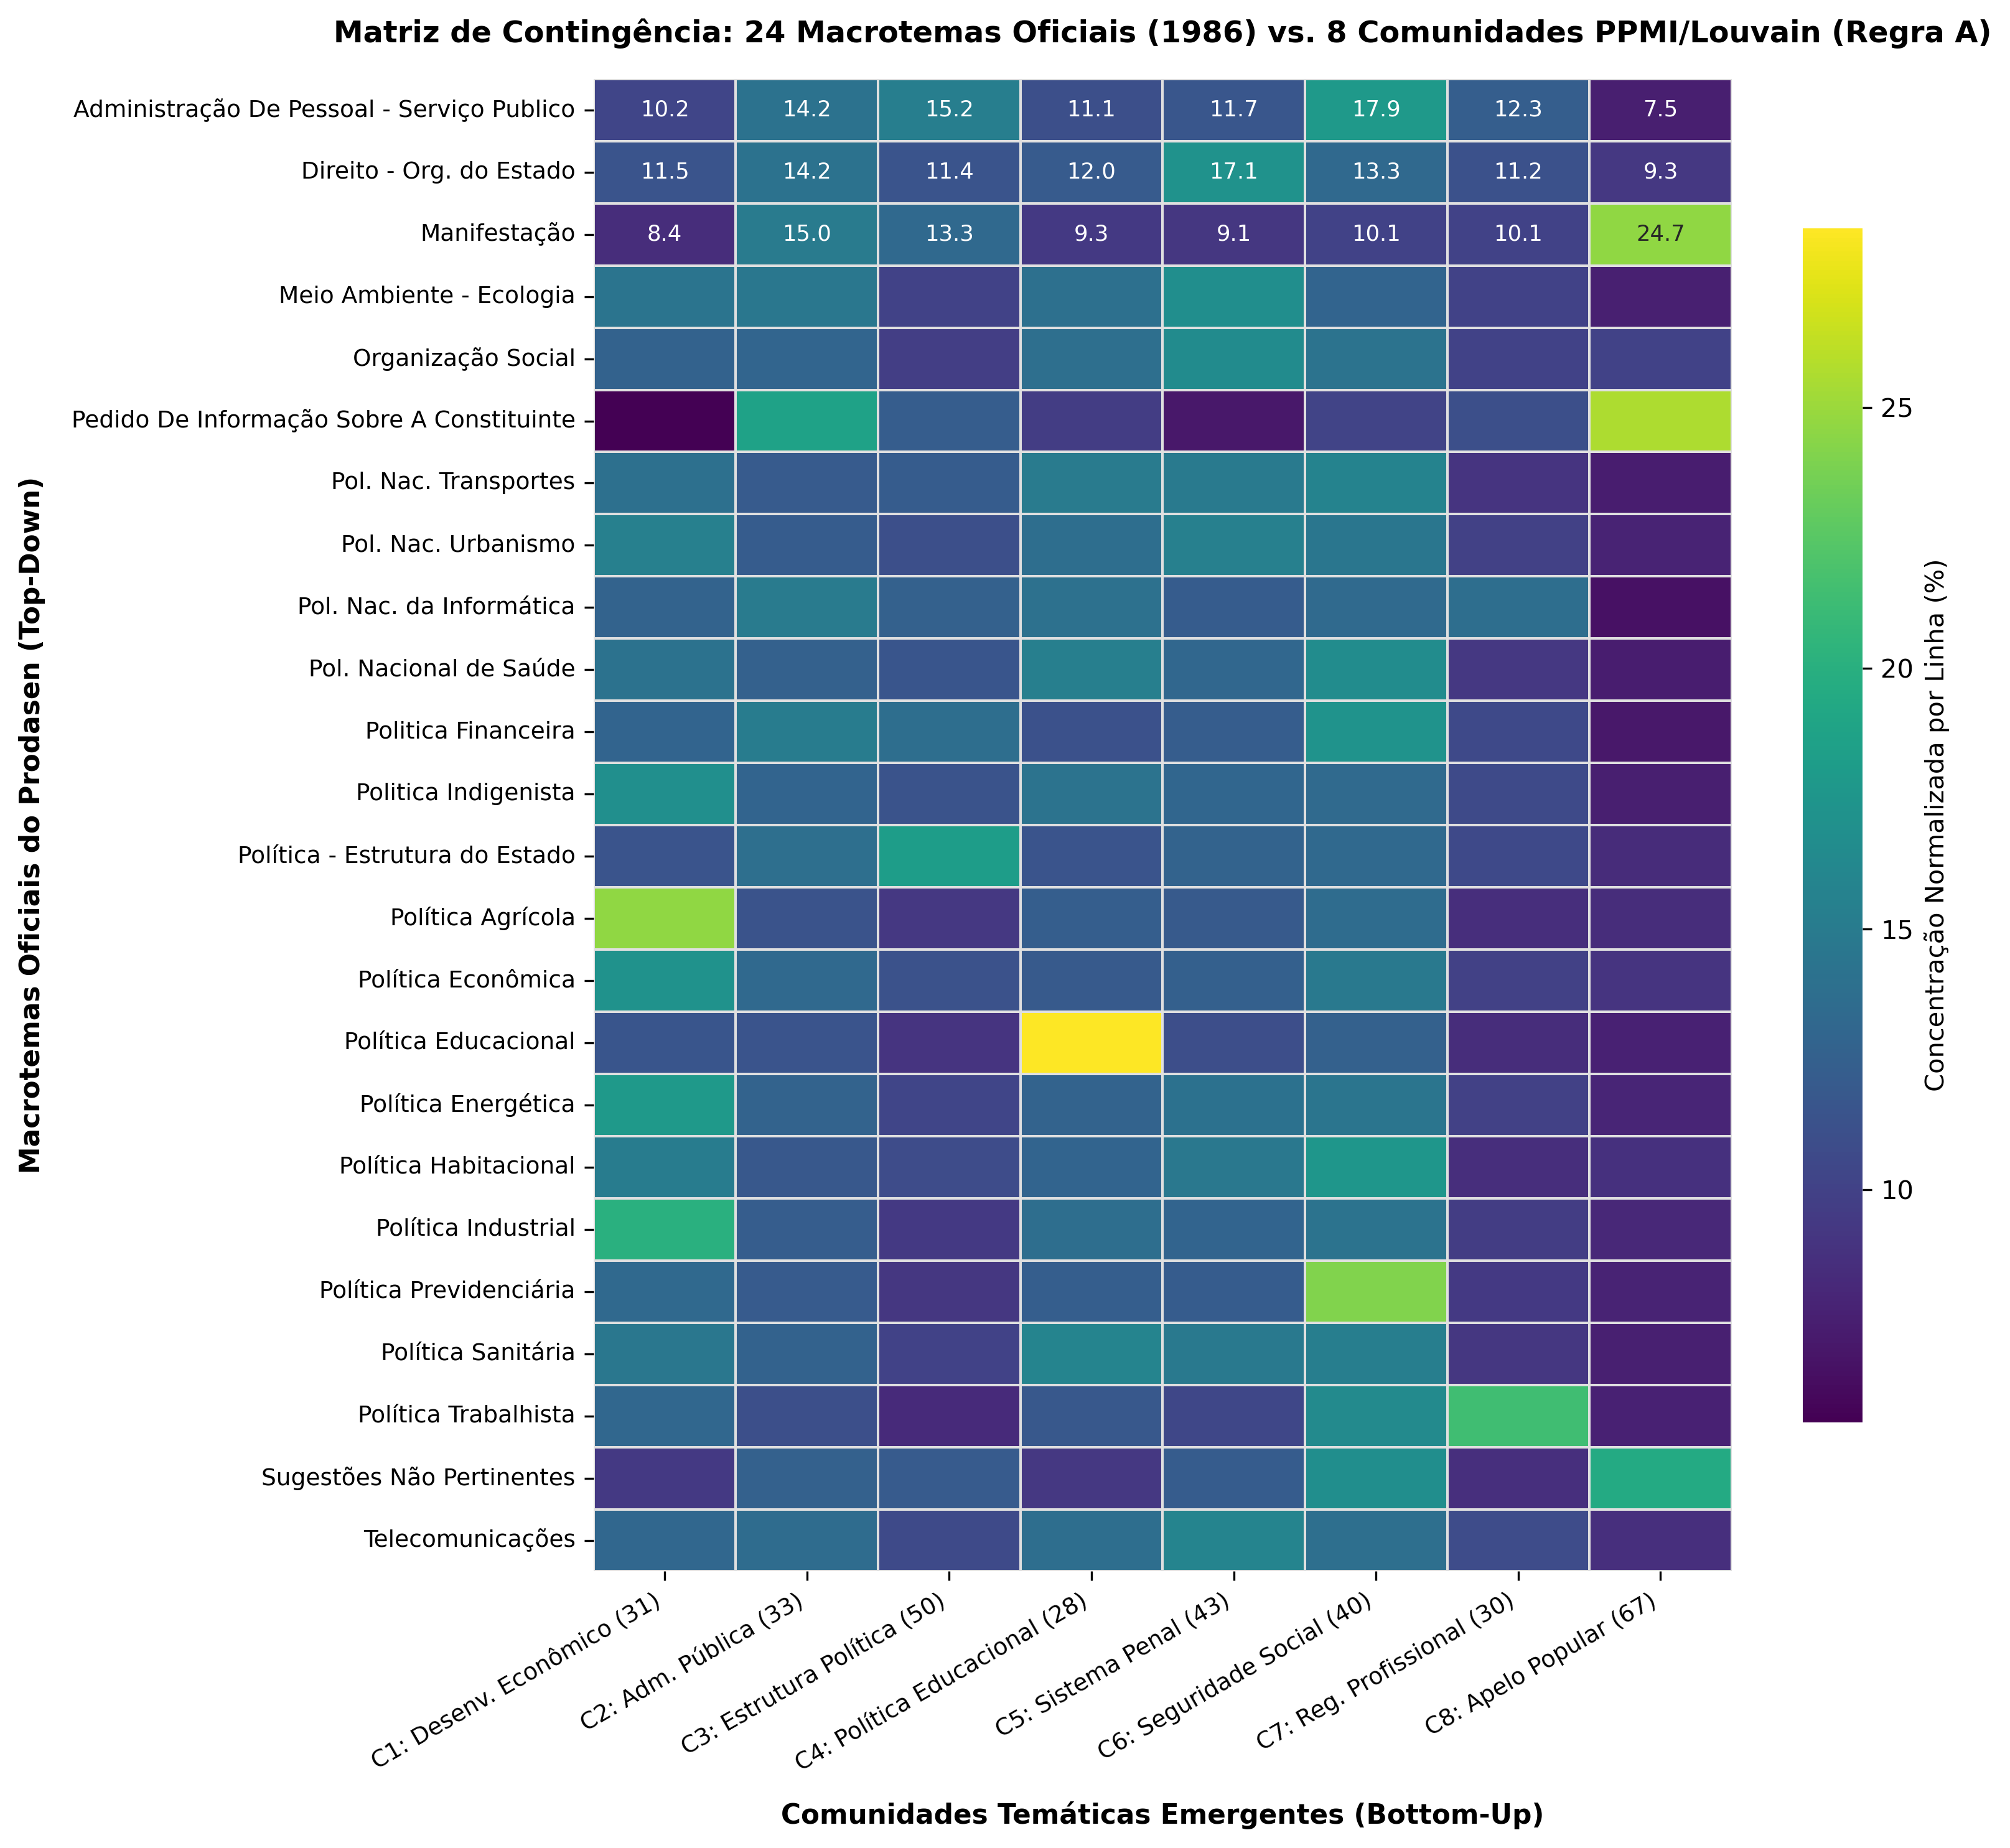
\includegraphics[width=0.85\textwidth]{heatmap_contingencia_brasnam.png}
\caption{Matriz de contingência normalizada (\%) entre os 24 temas oficiais do Prodasen (\textit{top-down}) e as 8 comunidades detectadas no grafo (\textit{bottom-up}) calculada pela Regra A.}
\label{fig:heatmap}
\end{figure}

O cruzamento quantitativo (Figura~\ref{fig:heatmap}) evidencia onde a taxonomia original de 1986 acertou e onde apresentou falhas de concepção:
\begin{itemize}
    \item \textbf{Alta convergência em Educação (C4), Estrutura Política (C3) e Regulação Profissional (C7):} O macrotema oficial \textit{Política Educacional} apresenta forte concentração na comunidade C4 ($28{,}4\%$). Da mesma forma, \textit{Política --- Estrutura do Estado} alinha-se prioritariamente à comunidade C3 ($18{,}2\%$), que separa de modo nítido a política representativa/eleitoral (C3) da máquina administrativa estatal (C2). Já \textit{Política Trabalhista} concentra sua maior afinidade na comunidade C7 ($21{,}4\%$), impulsionada pela expressiva mobilização corporativa dos detetives particulares --- nossa auditoria identificou \textbf{2.060 cartas} (2,8\% de todo o acervo da Constituinte!) contendo o termo \textit{``detetive''}.
    \item \textbf{Fusão orgânica da Seguridade Social (C6) e do Desenvolvimento Econômico (C1):} Enquanto o Prodasen separou \textit{Política Previdenciária}, \textit{Política Nacional de Saúde} e \textit{Política Habitacional}, os cidadãos articularam previdência, saúde, habitação e salário mínimo de forma indissociável na comunidade C6 (que captura $24{,}1\%$ de Previdência, $17{,}6\%$ de Habitação e $16{,}6\%$ de Saúde). Analogamente, C1 unifica \textit{Política Agrícola} ($24{,}6\%$), \textit{Política Industrial} ($20{,}1\%$), \textit{Política Energética} ($17{,}8\%$) e \textit{Política Econômica} ($17{,}1\%$).
    \item \textbf{A invisibilização da Segurança Pública (C5) no catálogo de 1986:} A comunidade C5 (\textit{Sistema Penal e Segurança}, 43 termos) absorve a maior fatia individual das duas maiores rubricas genéricas do Prodasen: \textit{Direito --- Organização do Estado} ($17{,}1\%$, que somava 25.243 cartas) e \textit{Organização Social} ($16{,}5\%$, com 23.555 cartas). Isso comprova que a segurança pública, o combate à violência e o debate penal constituíam uma das maiores preocupações populares de 1986--1987, mas foram diluídos pelo Prodasen dentro de macrotemas jurídicos e sociais genéricos, ao passo que temas com poucas centenas de cartas (como \textit{Informática}, com 282 registros) receberam categorias exclusivas.
    \item \textbf{Reinterpretação de ``Sugestões Não Pertinentes'' (C8):} As categorias oficiais \textit{Pedido de Informação sobre a Constituinte} ($25{,}7\%$), \textit{Manifestação} ($24{,}7\%$) e \textit{Sugestões Não Pertinentes} ($19{,}4\%$) convergem fortemente para a comunidade C8 (\textit{Apelo Popular, Críticas e Manifestações}). Isso demonstra que milhares de cartas rotuladas burocraticamente como ``não pertinentes'' pela triagem de 1986 não eram ruído sem sentido, mas sim relatos pessoais de fome, desemprego, carestia e apelos diretos às autoridades (como o presidente José Sarney) e a Deus.
\end{itemize}

\paragraph{Robustez frente à Atribuição Discreta (Regra B).}
A alocação de cada carta exclusivamente à comunidade de maior afinidade semântica (Regra B) confirmou alinhamento perfeito nos eixos dominantes (\textit{Educação} $\to$ C4 com $38{,}1\%$; \textit{Estrutura do Estado} $\to$ C3 com $44{,}4\%$; \textit{Trabalhista} $\to$ C7 com $40{,}3\%$). Contudo, o efeito \textit{winner-takes-all} concentrou cartas longas em agrupamentos maiores (erro médio absoluto de 8,55 p.p.), comprovando a superioridade da Regra A ao capturar a multitematicidade popular real.

\section{Conclusões e Trabalhos Futuros}

Este trabalho apresentou o processo completo de restauração, padronização e disponibilização pública da base histórica SAIC (72.719 cartas enviadas à Assembleia Nacional Constituinte de 1988, mapeadas em 64.869 cidadãos únicos), seguido de uma reanálise temática \textit{bottom-up} via redes de coocorrência de termos ponderadas por PPMI e particionadas pelo algoritmo de Louvain. Tanto a base higienizada quanto os scripts utilizados estão disponíveis em \repolink.

Demonstrou-se que a modelagem em nível de palavras ponderada por PPMI ($\text{min\_df} = 2{,}0\%$, percentil 95) desfaz o bloco indiferenciado de cartas multitemáticas e atinge alta modularidade ($Q = 0,6363$) em uma única componente conexa, revelando 8 grandes eixos discursivos. O confronto quantitativo e qualitativo com o catálogo de 24 temas do Prodasen evidenciou que a classificação oficial de 1986 sofreu de excessiva especialização técnica em áreas de baixa demanda popular e de grave falta de granularidade em demandas sociais críticas --- notadamente ao omitir uma categoria própria para \textbf{Sistema Penal e Segurança Pública} e ao rotular desabafos sociais sobre fome e desemprego como \textit{Sugestões Não Pertinentes}.

Como trabalhos futuros, propõe-se: (i) a aplicação recursiva de algoritmos de detecção de comunidades (Louvain e Leiden) sobre os subgrafos de cada uma das 8 comunidades para extrair subtemas hierárquicos e compará-los aos 1.308 itens da coluna \textit{Indexação}; (ii) o aprimoramento da etapa de normalização morfológica com lematizadores neuronais contextualizados; e (iii) o cruzamento das 8 comunidades temáticas com os atributos sociodemográficos e regionais dos 64.869 cidadãos identificados pela nova variável \textit{ID Pessoa}.

\bibliographystyle{sbc}
\begin{thebibliography}{99}

\bibitem[Agência Senado 2024]{agenciasenado2024}
Agência Senado (2024).
\newblock A Constituição dos Sonhos: conheça a história das 72 mil cartas enviadas por cidadãos à Assembleia Nacional Constituinte e saiba como consultá-las.
\newblock Disponível em: \url{https://www12.senado.leg.br/noticias/constituicao-dos-sonhos/}.

\bibitem[Blondel et~al. 2008]{blondel2008}
Blondel, V.~D., Guillaume, J.-L., Lambiotte, R., and Lefebvre, E. (2008).
\newblock Fast unfolding of communities in large networks.
\newblock {\em Journal of Statistical Mechanics: Theory and Experiment}, 2008(10):P10008.

\bibitem[Church and Hanks 1990]{church1990}
Church, K.~W. and Hanks, P. (1990).
\newblock Word association norms, mutual information, and lexicography.
\newblock {\em Computational Linguistics}, 16(1):22--29.

\bibitem[Erz 2026]{erz2026}
Erz, H. (2026).
\newblock Measuring issue-level polarization in congressional speech using community detection algorithms.
\newblock {\em Network Science}, 14:e28.

\bibitem[Girvan and Newman 2002]{girvan2002}
Girvan, M. and Newman, M.~E. (2002).
\newblock Community structure in social and biological networks.
\newblock {\em Proceedings of the National Academy of Sciences}, 99(12):7821--7826.

\bibitem[Hotho et~al. 2005]{hotho2005}
Hotho, A., Nürnberger, A., and Paa{\ss}, G. (2005).
\newblock A brief survey of text mining.
\newblock {\em Journal for Language Technology and Computational Linguistics}, 20(1):19--62.

\bibitem[Kim et~al. 2011]{kim2011}
Kim, Y., Choi, T.~Y., Yan, T., and Dooley, K. (2011).
\newblock Structural investigation of supply networks: A social network analysis approach.
\newblock {\em Journal of Operations Management}, 29(3):194--211.

\bibitem[Levenshtein 1966]{levenshtein1966}
Levenshtein, V.~I. (1966).
\newblock Binary codes capable of correcting deletions, insertions, and reversals.
\newblock {\em Soviet Physics Doklady}, 10(8):707--710.

\bibitem[Macanovic 2022]{macanovic2022}
Macanovic, A. (2022).
\newblock Text mining for social science -- the state and the future of computational text analysis in sociology.
\newblock {\em Social Science Research}, 108:102784.

\bibitem[Monclaire et~al. 1991]{monclaire1991}
Monclaire, S. et~al. (1991).
\newblock {\em A Constituição desejada: (SAIC: as 72.719 sugestões enviadas pelos cidadãos brasileiros à Assembleia Nacional Constituinte)}.
\newblock Senado Federal, Brasília.

\bibitem[Navarro 2001]{navarro2001}
Navarro, G. (2001).
\newblock A guided tour to approximate string matching.
\newblock {\em ACM Computing Surveys}, 33(1):31--88.

\bibitem[Rule et~al. 2015]{rule2015}
Rule, A., Cointet, J.-P., and Bearman, P.~S. (2015).
\newblock Lexical shifts, substantive changes, and continuity in State of the Union discourse, 1790--2014.
\newblock {\em Proceedings of the National Academy of Sciences}, 112(35):10837--10844.

\bibitem[Schaeffer 2007]{schaeffer2007}
Schaeffer, S.~E. (2007).
\newblock Graph clustering.
\newblock {\em Computer Science Review}, 1(1):27--64.

\bibitem[Senado Federal 1988]{senado1988}
Senado Federal (1988).
\newblock Base SAIC -- Sugestões da população para a Assembleia Nacional Constituinte de 1988.
\newblock Brasília.

\bibitem[Tan et~al. 1999]{tan1999}
Tan, A.-H. et~al. (1999).
\newblock Text mining: The state of the art and the challenges.
\newblock In {\em Proceedings of the PAKDD 1999 Workshop on Knowledge Discovery from Advanced Databases}, pages 65--70.

\bibitem[Tsai et~al. 2022]{tsai2022}
Tsai, W.-C. et~al. (2022).
\newblock Natural language processing and network analysis in patients withdrawing from life-sustaining treatments: a retrospective cohort study.
\newblock {\em BMC Palliative Care}, 21(1):225.

\end{thebibliography}

\end{document}
